% Modified from: https://www.integral-domain.org/lwilliams/Resources/TikzImg/dodecagraph.tex

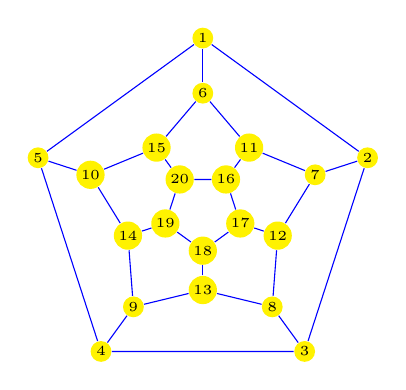
\begin{tikzpicture}[
  baseline,
  every node/.style = {
    circle,
    fill=yellow,
    node font=\tiny,
    inner sep=1pt,
    minimum size=2pt
  },
  uedge/.style={draw=blue}
]
    \foreach \x [
      evaluate=\x as \xo using {int(mod(6-\x,5)+1)},
      evaluate=\x as \xi using {int(mod(6-\x,5)+6)},
      evaluate=\x as \xii using {int(mod(5-\x,5)+11)},
      evaluate=\x as \xiii using {int(mod(5-\x,5)+16)},
    ] in {0,1,2,3,4}{
        \node (o\x) at (18+\x*72:2.2cm) {\xo};
        \node (i\x) at (18+\x*72:1.5cm) {\xi};
        \node (ii\x) at (54+\x*72:1cm) {\xii};
        \node (iii\x) at (54+\x*72:0.5cm) {\xiii};
    }
    \foreach \x in {0,1,2,3,4}{
        \path[uedge] (o\x) edge (i\x);
        \path[uedge] (ii\x) edge (iii\x);
    }
    \path[uedge] (o0)--(o1)--(o2)--(o3)--(o4)--(o0);
    \path[uedge] (iii0)--(iii1)--(iii2)--(iii3)--(iii4)--(iii0);
    \path[uedge] (i0)--(ii0)--(i1)--(ii1)--(i2)--(ii2)--(i3)--(ii3)--(i4)--(ii4)--(i0);
\end{tikzpicture}